\section{AKLT model, Entanglement Entropy I}
We discuss one more model of a 1-D SPT; the AKLT (Affleck-Kennedy-Lieb-Tasaki) model. This was (arguably) the first SPT phase that was understood.

\subsection{Defining the model}
We now consider a chain of qutrits/spin-1 particles.

\begin{center}
    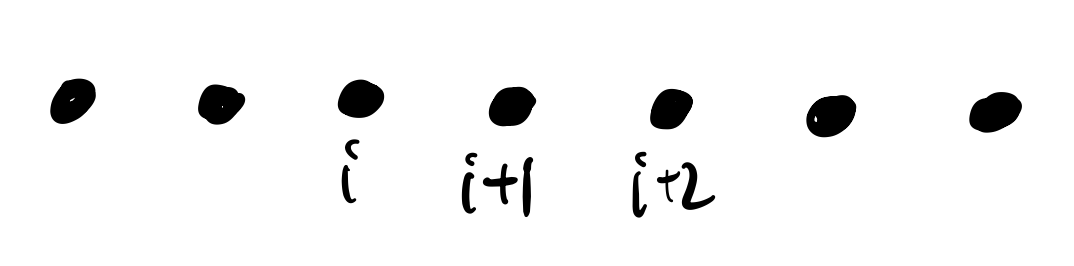
\includegraphics[scale=0.35]{Lectures/Images/lec15-spinchain.png}
\end{center}

The Hamiltonian takes the form:
\begin{equation}
    H = \sum_i P_2(\v{S}_i + \v{S}_{i+1})
\end{equation}
what is this? This is a projection that acts on two neighbouring sites, and projects it onto states with total spin 2 (the projection onto the subspace with eigenvalues $s(s+1) = 2(2+1) = 6$).  This projector has a reasonably nice form:
\begin{equation}
    H = \sum_i \left[\frac{1}{2}\v{S}_i \cdot \v{S}_{i+1} +\frac{1}{6}(\v{S}_i\cdot\v{S}_{i+1})^2 + \frac{1}{3}\right]
\end{equation}
Note that any rotation-symmetric quantity can be written as a function of $\v{S}_i \cdot \v{S}_{i+1}$, which is what we see above. 

% There are three possible projectors we could write down, $P_0, P_1, P_2$, the third is not independent (is just $\II - P_i - P_j$) so this motivates why we just get the terms that we do.

We focus on the (global) $SO(3)$ symmetry of the model. Why is it a nontrivial phase in the presence of this symmetry? Let us write down a unitary operator for each rotation matrix in $SO(3)$:
\begin{equation}
    U(R(\theta, \hat{\v{n}})) = \prod_k e^{-i\theta \v{S}_k \cdot \hat{\v{n}}}
\end{equation}

Note that each site transforms under a linear (\emph{not} projective) representation of $SO(3)$. This is because they are spin-1 (this is the analog of each site of our cluster state transforming under a linear representation of $\mathbb{Z}_2 \times \mathbb{Z}_2$). When we look at the boundary, we will see that the symmetry acts on the boundary via projective representations\footnote{and this motivates why $SO(3)$ rather than $SU(2)$, as $SU(2)$ does not have projective representations.}

\subsection{Constructing the ground state}
One can show that $H$ has a unique ground state $\ket{\Omega}$ and a gap in infinite (or periodic) chain. This ground state has a simple picture; we represent each spin-1 as two spin-1/2s in a spin-triplet state:
\begin{equation}
    \begin{split}
        \ket{+} &\leftrightarrow \ket{\uparrow\uparrow}
        \\ \ket{0} &\leftrightarrow \frac{\ket{\uparrow\downarrow} + \ket{\downarrow\uparrow}}{\sqrt{2}}
        \\ \ket{-} &\leftrightarrow \ket{\downarrow\downarrow}
    \end{split}
\end{equation}
We have no singlet state - the singlet state for the spin-1/2s does not correspond to a physical state in the real spin-1 system. Why did we do this weird rewriting in terms of virtual spin-1/2s? The ground states will have a very simple form in this notation:

\begin{center}
    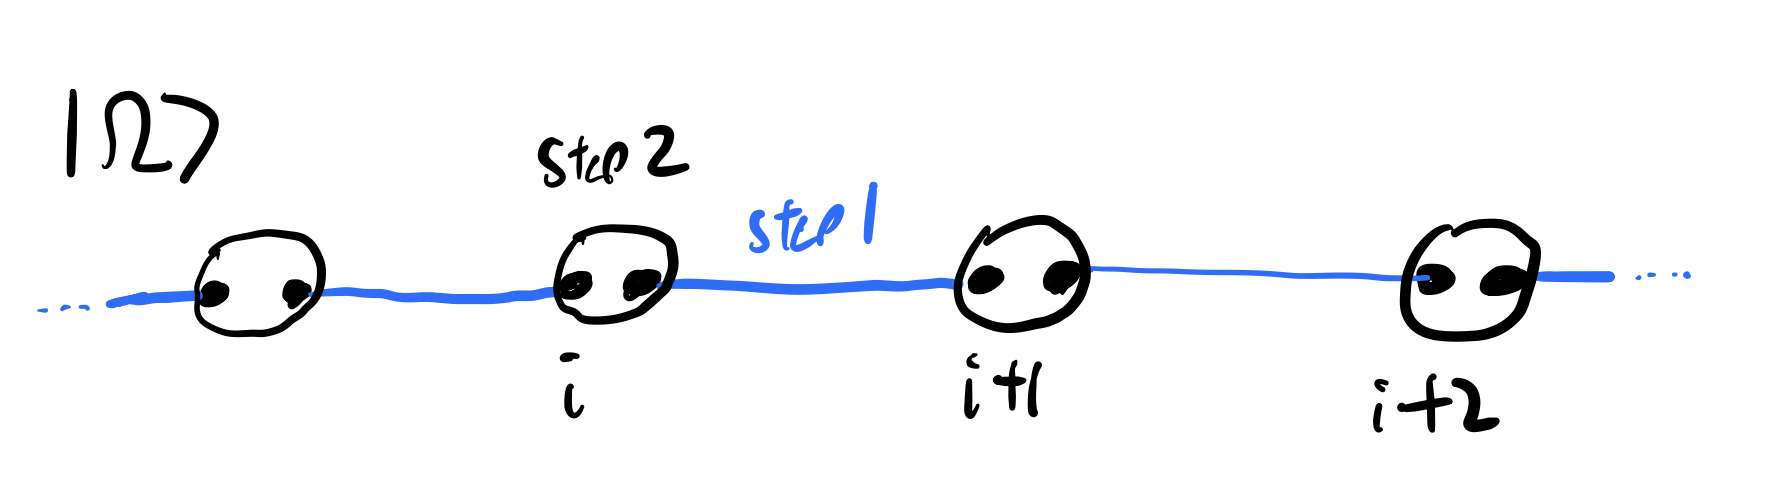
\includegraphics[scale=0.35]{Lectures/Images/lec15-AKLTGS.png}
\end{center}

The blue lines connecting the fictituous spin-1/2 particles on neighbouring sites corresponds to the projection onto the spin singlet state $\frac{\ket{\uparrow\downarrow} - \ket{\downarrow\uparrow}}{\sqrt{2}}$. This alone is not good, because we are taken out of the space of physical spin-1 states. So, after the singlet projection, we apply the black circles, which are a projection onto the spin-triplet subspace for each ``true'' spin-1 site.

To see that $\ket{\Omega}$ is indeed the ground state of $H$, note that we have a maximum spin of $1/2$ from each of the boundary spins, and then a spin of 0 from the singlet (note that this analysis seems like it happened before the triplet projection - but since the triplet projection is $SU(2)$ symmetric, it doesn't change the spin, so this is justified).

\begin{center}
    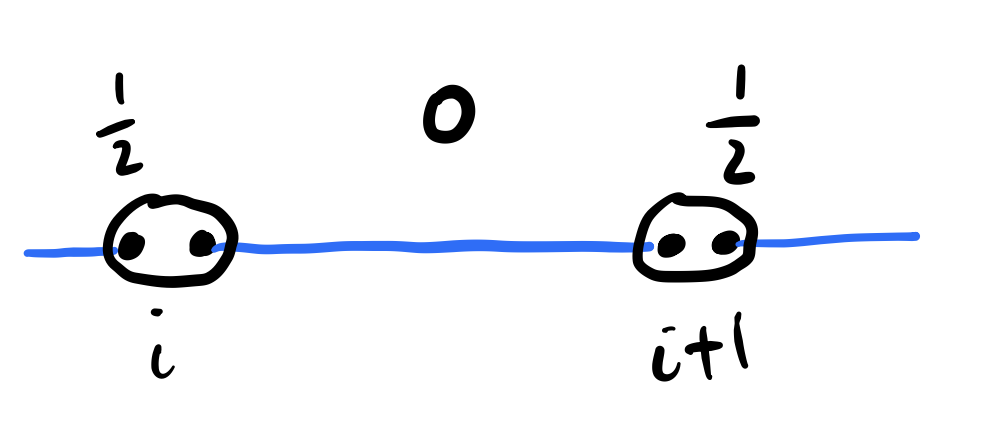
\includegraphics[scale=0.35]{Lectures/Images/lec15-AKLTspin.png}
\end{center}

To, the total spin of $i, i+1$ is bounded above by $\frac{1}{2} + 0 + \frac{1}{2} = 1$. So:
\begin{equation}
    P(\v{S}_i + \v{S}_{i+1})\ket{\Omega} = 0
\end{equation}
which allows us to indeed conclude that this is a ground state.

\subsection{Physics of the boundary}
Let's truncate the Hamiltonian to fit on our open chain:
\begin{equation}
    H = \sum_{i=1}^{N-1}P_2(\v{S}_i + \v{S}_{i+1})
\end{equation}
We can now see immediately that there are 4 degenerate ground states:

\begin{center}
    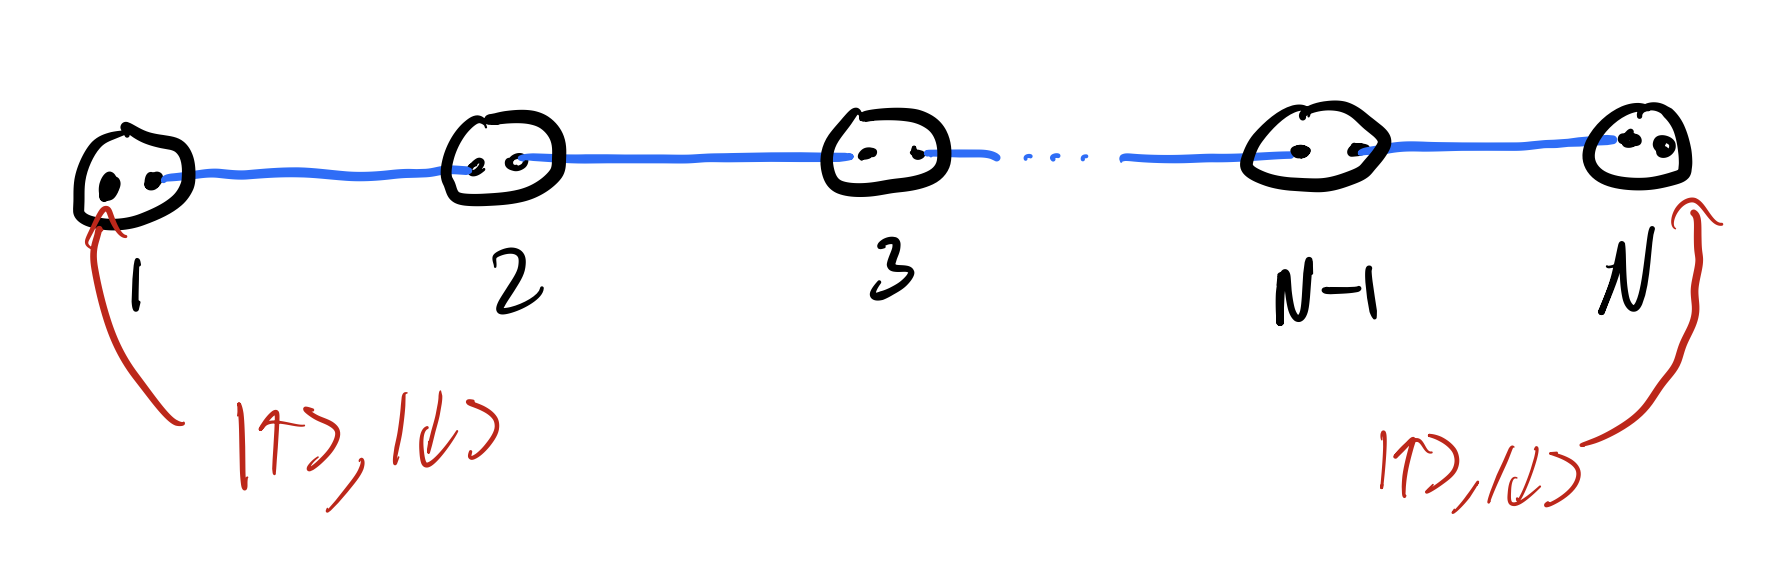
\includegraphics[scale=0.35]{Lectures/Images/lec15-AKLTboundary.png}
\end{center}

The boundary spins are now free to be up or down, and the same construction of singlet/triplet projection yields that all four choices of $\uparrow/\downarrow$ gives a ground state.

The degeneracy is just like the cluster state! The cluster state was a commuting projector Hamiltonian/solvable but less intuitive - here we have no commuting projector Hamiltonian but the picture is more intuitive/not solvable. But the physics is the same.

From the picture, it is clear that we have effective qubits on the left/right boundaries of the system (this interesting! We started with qutrits and now the effective DoFs are qubits), and that they transform like spin-1/2 under $SO(3)$. While spin-1 is a linear representation of $SO(3)$, spin-1/2 is a projective representation of $SO(3)$; we again see that the symmetry acts via projective representation on the boundaries of the system.

\subsection{Generalizations}

Note that there is a similar structure for other 1D (bosonic) SPT phases. The sites transform under a linear representation of $G$. But, when we define the system on an open chain, we get edge states that transform under a projective representation of $G$. The physical consequence of this structure is you get a robust GSD in an open chain.

We can also consider higher-dimensional SPT phases. For example, consider a 2D spin lattice with a boundary. In this case, we find that the symmetry action on the edge degrees of freedom is anomalous - roughly speaking, it means the symmetry acts in a way that is impossible to get for a lower-dimensional system. In 1-D the symmetry action at the boundary gave us GSD. In higher dimensions, it roughly gives us robust gapless modes; even though we may have a gap in the bulk at the boundary the gap closes.

\subsection{Schmidt Decomposition}
We now move to the last topic of the course, about entanglement measures. To this end let's review notions of the Schmidt decomposition and entanglement entropy.

Consider a state $\ket{\Psi}$ defined on a collection of qubits, partitioned into two subsets $A, A^c$.

\begin{center}
    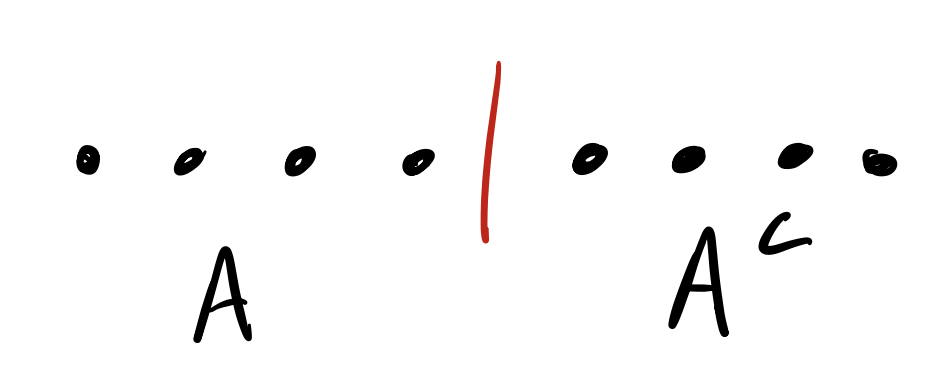
\includegraphics[scale=0.35]{Lectures/Images/lec15-subsystems.png}
\end{center}

Then, the Schmidt decomposition of $\ket{\Psi}$ is:
\begin{equation}
    \ket{\Psi} = \sum_i \lambda_i \ket{\psi^i_A}\otimes \ket{\psi^i_{A^c}}
\end{equation}
for $\lambda_i \geq 0$. $\set{\ket{\psi^i_A}}_i, \set{\ket{\psi^i_{A^c}}}_i$ are orthonormal bases for $\mathcal{H}_A, \mathcal{H}_{A^c}$. Normalization tells us that:
\begin{equation}
    \sum_i \abs{\lambda_i}^2 = 1.
\end{equation}
We call the $\lambda_i$s Schmidt coefficients. These are unique up to reordering. We call the $\ket{\psi^i_A}, \ket{\psi^i_{A^c}}$ Schmnidt states, which are unique up to phases if the $\lambda_i$ are non-degenerate (in which case they would be unique up to unitary mixing of the states with the same Schmidt coefficient).

This all follows from singular value decomposition of matrices - same thing with a different name.

Note that $\set{\lambda_i}$ characterize the entanglement between $A, A^c$. We can see this from two properties:
\begin{enumerate}
    \item $\set{\lambda_i}$ are invariant under $\ket{\Psi} \to U_AU_{A^c}\ket{\Psi}$, where $U_{A}, U_{A^c}$ are unitaries that act on $A, A^c$ only. We can see that the unitary transformation would only change/rotate the basis of Schmidt states, but the coefficients would be preserved.
    \item $\set{\lambda_1 = 1, \text{others} = 0} \iff$ $\ket{\Psi}$ is a product state $\ket{\Psi} = \ket{\psi_A} \otimes \ket{\psi_{A^c}}$. Other values of $\lambda_i$ imply that the state is entangled.
\end{enumerate}

\subsection{Entanglement Entropy}
Let $\rho = \dyad{\Psi}{\Psi}$. Then, we define the Von Neumann entanglement entropy of $A$ as:
\begin{equation}
    S(\rho_A) = -\Tr(\rho_A\log \rho_A)
\end{equation}
where $\rho_A$ is the reduced density operator:
\begin{equation}
    \rho_A = \Tr_{A^c}(\rho)
\end{equation}
which is the reduced density operator.

Let's discuss the relationship between the Von Neumann entanglement entropy and the Schmidt coefficients $\set{\lambda_i}$. If we look at the expression for the Schmidt decomposition of $\ket{\Psi}$ across $A/A^c$ we can see that:
\begin{equation}
    \rho_A = \sum_i \abs{\lambda_i}^2\dyad{\psi^i_A}{\psi^i_A}
\end{equation}
The eigenvalues of $\rho_A$ are then $\set{\abs{\lambda_i}^2}$, and so:
\begin{equation}
    S(\rho_A) = -\sum_i \abs{\lambda_i}^2\log(\abs{\lambda_i}^2)
\end{equation}
indeed the entropy depends on the Schmidt coefficients, so $S(\rho_A)$ is indeed an entanglement measure. Because we get the same $\lambda_i$s whether we work with $A$ or $A^c$, an immediate (and intuitive) consequence is:
\begin{equation}
    S(\rho_A) = S(\rho_{A^c}).
\end{equation}

Properties of $S(\rho_A)$:
\begin{enumerate}
    \item $S(\rho_A)$ is invariant under $\rho \to U_A U_{A^c} \rho U^\dag_{A^c}U_{A^c}$ which is clear because it depends on the $\set{\lambda_i}$s, which are invariant under such a unitary that does not cross the bipartition.
    \item $S(\rho_{A_1} \otimes \rho_{A_2}) = S(\rho_{A_1}) + S(\rho_{A_2})$ for regions $A_1, A_2$.
    \item $0 \leq S(\rho_A) \leq \log(\text{min}(\dim \mathcal{H}_A, \text{dim} \mathcal{H}_{A^c}))$, where $\text{dim} \mathcal{H}_A$ is the dimension of the Hilbert space associated with $A$. This is achieved by setting all of the Schmidt coefficients to be equal weight (and corresponds to the maximally mixed state).
    \item $S(\rho_A) = 0 \iff \ket{\Psi} = \ket{\psi_A} \otimes \ket{\psi_{A^c}}$, $S(\rho_A) \neq 0 \iff \ket{\Psi}$ entangled.
    \item $S(\rho_{AB}) + S(\rho_{BC}) \geq S(\rho_{ABC}) + S(\rho_B)$ for any regions $A, B, C$ with $AB = A\cup B, BC = B \cup C$, $ABC = A \cup B \cup C$. This is the strong subadditivity property, and a very deep and nontrivial result, and motivates this entanglement measures over other ones.
\end{enumerate}

Next class we will discuss entanglement entropy in many-body systems.